%%%%%%%%%%%%%%%%%%%%%%%%%%%%%%%%%%%%%%%%%%%%%%%%%%%%%%%%%%%%%%%%%%%%%%%%
%    INSTITUTE OF PHYSICS PUBLISHING                                   %
%                                                                      %
%   `Preparing an article for publication in an Institute of Physics   %
%    Publishing journal using LaTeX'                                   %
%                                                                      %
%    LaTeX source code `ioplau2e.tex' used to generate `author         %
%    guidelines', the documentation explaining and demonstrating use   %
%    of the Institute of Physics Publishing LaTeX preprint files       %
%    `iopart.cls, iopart12.clo and iopart10.clo'.                      %
%                                                                      %
%    `ioplau2e.tex' itself uses LaTeX with `iopart.cls'                %
%                                                                      %
%%%%%%%%%%%%%%%%%%%%%%%%%%%%%%%%%%
%
%
% First we have a character check
%
% ! exclamation mark    " double quote  
% # hash                ` opening quote (grave)
% & ampersand           ' closing quote (acute)
% $ dollar              % percent       
% ( open parenthesis    ) close paren.  
% - hyphen              = equals sign
% | vertical bar        ~ tilde         
% @ at sign             _ underscore
% { open curly brace    } close curly   
% [ open square         ] close square bracket
% + plus sign           ; semi-colon    
% * asterisk            : colon
% < open angle bracket  > close angle   
% , comma               . full stop
% ? question mark       / forward slash 
% \ backslash           ^ circumflex
%
% ABCDEFGHIJKLMNOPQRSTUVWXYZ 
% abcdefghijklmnopqrstuvwxyz 
% 1234567890
%
%%%%%%%%%%%%%%%%%%%%%%%%%%%%%%%%%%%%%%%%%%%%%%%%%%%%%%%%%%%%%%%%%%%
%
\documentclass[12pt]{iopart}
\newcommand{\gguide}{{\it Preparing graphics for IOP Publishing journals}}
%Uncomment next line if AMS fonts required
%\usepackage{iopams} 


\usepackage{ amssymb }
\usepackage{graphicx}           % Import Pictures + PDFs
\usepackage[svgnames]{xcolor}   % Enabling colors by their 'svgnames'
\usepackage{ulem}
\definecolor{fzjblue}{HTML}{005B81}
\definecolor{light-gray}{gray}{0.97}
\definecolor{mygreen}{rgb}{0,0.6,0}
\usepackage{listings} %  See: https://en.wikibooks.org/wiki/LaTeX/Source_Code_Listings
\lstset{
  language=Python,
  backgroundcolor=\color{light-gray},   % choose the background color; you must add \usepackage{color} or \usepackage{xcolor}
  basicstyle=\linespread{1}\footnotesize,        % the size of the fonts that are used for the code
  commentstyle=\color{mygreen},
  frame=single,
  keywordstyle=\color{blue},       % keyword style
  tabsize=4,	                   % sets default tabsize to 2 spaces
  rulecolor=\color{light-gray},
}

\newcommand{\python}[0]{\texttt{Python} }
\newcommand{\abs}[1]{\left\vert #1 \right\vert}

\begin{document}

\title[A primer to numerical simulations]{A primer to numerical simulations: The perihelion
motion of Mercury}

\author{I. Hammer, C. Hanhart, C. K\"orber and C. M\"uller}

\address{Forschungszentrum J\"ulich}
\ead{c.hanhart@fz-juelich.de}
\vspace{10pt}
%\begin{indented}
%\item[]February 2014
%\end{indented}

\begin{abstract}
Numerical simulations are playing an increasingly important role in modern science. In this work it is
suggested to use a numerical study of the famous perihelion motion of the planet Mercury (one of the prime observables
supporting Einsteins General Relativity) as a test case to teach numerical simulations to high school students.
The paper includes details about the development of the code as well as a discussion of the visualization 
of the results. In addition a method is discussed how to estimate the size of the effect a priori. 
\end{abstract}

% Uncomment for PACS numbers
%\pacs{00.00, 20.00, 42.10}
%
% Uncomment for keywords
%\vspace{2pc}
%\noindent{\it Keywords}: XXXXXX, YYYYYYYY, ZZZZZZZZZ
%
% Uncomment for Submitted to journal title message
%\submitto{\JPA}
%
% Uncomment if a separate title page is required
%\maketitle
% 
% For two-column output uncomment the next line and choose [10pt] rather than [12pt] in the \documentclass declaration
%\ioptwocol
%



\section{Introduction}

Numerical simulations play a key role in modern physics for they allow one to tackle theoretical problems
not accessible otherwise, e.g., since there are too many particle participating in the system (as in
simulations for weather predictions) or the interactions are too complicated to allow for a systematic,
perturbative approach (as in theoretical descriptions of nuclear particles at the fundamental level). 
 The goal of this paper is it to
introduce a project that could be used to make numerical simulations themselves the topic of the class.
On the example of the perihelion motion of the planet Mercury the students are supposed to get in touch with
\begin{itemize}
\item the importance of differential equations in theoretical physics;
\item the numerical implementation of Newtonian dynamics;
\item systematic tests and optimization of computer codes;
\item effective tools to estimate the result a priori as an important cross check;
\item the visualization of numerical results using V-Phython.
\end{itemize}
The course as well as this paper is structured as follows: after an introduction to Newtonian dynamics and the 
concepts of differential equations their discretization is discussed based on Newtons law of gravitation and possible
extensions thereof. Afterwards the visualization of the resulting trajectories using V-Phython is introduced and
applied to the problem at hand. In particular tools are developed to extract the relevant quantity from the result
of the simulation.
Finally the principle of dimensional analysis is presented as a tool to cross check, if the results of the simulation
are sensible.

We are convinced that in order to excite the students for numerical simulations it is compulsory to
demonstrate their power on an example that they catches their interest. This purpose is served 
perfectly by the case chosen here, since Einsteins equations of General Relativity are fascinating to
a very broad public. While their detailed study needs deeper knowledge in Differential Geometry, for
the study outlined here very little math is necessary, such that high school students from about 
10$^{\rm th}$ grade up should benefit from it. This was already demonstrated in the
'Sch\"ulderakademie Teilchenphysik', where an early version of this course was tested successfully 
on a goup of 10 German high school students from 10$^{\rm th}$ to 13$^{\rm th}$ grade.

\section{Trajectories, velocities, accelerations and Newtons second law}
\label{sec:tva}

We can say that we understand a physical system, if we can demonstrate that the assumed force leads to the trajectories
observed. In other words, we need to show that we can calculate the location in space of the object of interest at any point
in time, once the initial conditions are fixed properly. If we can neglect the finite size of this object (and
in particular its orientation in space) the location is parametrized
by a single three vector $\vec x(t)$. As will become clear below in order to describe and control the dynamics of a physical
object in addition we need to be able to calculate its velocity, $\vec v(t)$, related to the location via
\begin{equation}\label{eq:x_update}
\vec x(t+\Delta t) = \vec x(t) + \vec v(t) \Delta t + ... \ , \label{eq:vdef}
\end{equation}
for some infinitesimally small $\Delta t$ and the acceleration, $\vec a(t)$ that describes the change of the velocity
\begin{eqnarray}\label{eq:v_update}
\vec v(t+\Delta t) = \vec v(t) + \vec a(t) \Delta t + ...\ . \label{eq:adef}
\end{eqnarray}
The dots in the above expressions indicate that there are in general additional terms that may be expressed with
higher powers in $\Delta t$, however, for sufficiently small $\Delta t$ those can be safely neglected.
Thus we may define the time derivative via
\begin{equation}
\vec v(t) = \lim_{\Delta t\to 0} \frac{\Delta \vec x(t)}{\Delta t} =: \frac{d\vec x(t)}{dt}  = \dot{\vec  x}(t) \ ,
\end{equation}
where $\Delta \vec x(t)=\vec x(t+\Delta t)-\vec x(t)$ and we introduced with the last expression a common short hand notation
for time derivatives. Analogously we get
\begin{eqnarray}
\vec a(t) &=& \lim_{\Delta t\to 0} \frac{\Delta \vec v(t)}{\Delta t} =: \frac{d\vec v(t)}{dt}  = \dot{\vec v}(t) \ , \\
 &=& \frac{d^2\vec x(t)}{dt^2}  = \ddot{\vec x}(t) \ ,
\end{eqnarray}
where we introduced in the second line the second derivative.

It was Newton who observed that if a body is at rest it will remain at rest, and if it is in motion it will remain in motion in a 
constant velocity in a straight line, unless it is acted upon by some force --- this is known as Newtons first law. 
Said differently: a force $\vec F$ shows up by changing the motion of some object. This is quantified in Newton's second law
\begin{equation}
\vec F(\vec x, t) = \frac{d}{dt}(m \vec v) \ .
\end{equation} 
If the mass does not change~\footnote{A well known example where $m$ does change with time is a 
rocket, whose mass decreases as the rocket rises.} with time this reduces to the well known
\begin{equation}
\vec F(\vec x) = m \vec a(t) = m\dot{\vec v}(t) = m\ddot{\vec{x}}(t) \ . \label{eq:newton2}
\end{equation} 
Note that in general the force could depend also on the time or the velocity. We here restrict ourselves to the
case relevant for our example where the force depends on the location only. 
Therefore, 
as soon as the force $\vec F(\vec x)$ is known for all $\vec x$ one can in principle calculate the trajectory, e.g. solving eq.~(\ref{eq:newton2})
for $\vec x(t)$.
Sometimes this requires some advanced knowledge in math, sometimes no closed form solution exists. However, alternatively 
one can calculate the whole trajectory
of some test body that experiences this force by a successive application of the rules 
given in Eqs.~(\ref{eq:vdef}) and (\ref{eq:adef}):
\begin{enumerate}
\item For a given time $t$, where $\vec x(t)$ and $\vec v(t)$ are known, use Eq.~(\ref{eq:newton2}) to calculate $\vec a(t)$.
\item Use Eq.~(\ref{eq:vdef}) to calculate $\vec x(t+\Delta t)$ and
\item then use Eq.~(\ref{eq:adef}) to calculate $\vec v(t+\Delta t)$.
\item Go back to (i) with $t\to t+\Delta t$.
\end{enumerate}
Clearly to initiate the procedure at some time $t_0$ both $\vec x(t_0)$ as well as $\vec v(t_0)$ must be known --- the 
trajectories depend on these initial conditions.~\footnote{In general a differential equation of $n^{\rm th}$ degree (where
the highest derivative is $n$) needs $n$ initial conditions specified. For $n=2$ those are often chosen as location and velocity
at some defined time, but also to pick two location at different times is possible. }

Clearly for this procedure to work $\Delta t$ must be sufficiently small. What this means depends on the process
studied. One way to estimate, if $\Delta t$ is small enough, is to verify, if the relation
\begin{equation}
|\vec v(t)| \gg \frac12|\vec a(t)|\Delta t = \frac{1}{2m}\vec F(\vec x)\Delta t\ . 
\label{eq:check}
\end{equation}
holds, since the next term neglected in Eq.~(\ref{eq:vdef}) reads $(1/2)a(t)(\Delta t)^2$.  Eq.~({\ref{eq:check}})
also shows that small (large) time steps are necessary (sufficient), if the force is strong (weak), since
the time steps need to be small enough that all changes induced by the force get resolved. Clearly,
a relation as Eq.~({\ref{eq:check}}) can only provide guidance and can not replace a careful numerical check of
the solutions: A valid result has to be insensitive the concrete value $\Delta t$ chosen --- in particular replacing
$\Delta t$ by $\Delta t/2$ should not change the result significantly.


\section{Example: General Relativity and the perihelion motion of Mercury}


For this concrete example the starting point for the force is Newtons law
of gravitation
\begin{equation}
\vec F_N(\vec x) = \frac{G_N m M_\odot}{r^2} \frac{\vec r}{r}\ ,
\end{equation}
where $G_N=6.67\times 10^{-11}$ m$^3$kg$^{-1}$s${-2}$ is the Newtonian constant of gravitation,
$m$ is the mass of Mercury and $M_\odot=2\times 10^{30}$ kg is the mass of the sun.
In addition $r=|\vec x(t)|$ denotes the distance between sun and Mercury, when we assume that the sun
is infinitely more heavy than the planet and located at the center of the coordinate system. 
Although this is not exact, since $m/M_\odot\sim 10^{-8}$ this is
a pretty good approximation. For later convenience we introduce the Schwarzschildradius of the sun
\begin{equation}
r_S=\frac{2G_N  M_\odot}{c^2} = 3 \ \mbox{km} \ ,
\end{equation}
where $c=3\times 10^8$ m/s denotes the speed of light.
Note the $r_S$ is the characteristic length scale of the gravitational field of the sun
for --- up to the prefactor --- one can not form another quantity with dimensions of a length from $G_N$, $M_\odot$ and
$c$. This is what we need $r_S$ for later in the discussion. That the Schwarzschild radius is
also an important quantity to characterize black holes is not relevant for the discussion
at hand.
With this Newtons second law reads 
\begin{equation}
\ddot{\vec x} = \frac{c^2}{2}\left(\frac{r_S}{r^2}\right) \ .
\label{eq:newton}
\end{equation}
%\begin{itemize}
%\item{\bf First task:}
%Now the students should implement the program outlined in Sec.~\ref{sec:tva} and visualize the resulting
%trajectories of Mercury for different start parameters.
%Why is it sufficient to work in two dimensions using simply 
%$\vec x(t)=(x(t),y(t))^T$?
% When the parameters are chosen appropriately close
%orbits should emerge that are fixed in time --- in particular the perihelion (the point of closest approach
%of planet and sun) stays fixed in space.
%\end{itemize}
In general an attractive force that vanishes at large distances leads,
 depending on the initial conditions,
  either to closed orbits or open orbits --- 
  in the latter case the planet simply disappears from the sun. Depending on time available
for the course  it might be helpful to explain to the students the origin of this, however, since the most
transparent reasoning needs an integration as well as the concept of angular momentum
not necessarily familiar to the whole class (details are given in the appendix {\bf to be done}), 
it appears in general more appropriate to work out together with the students 
that a moving body can not be kept by a force if its momentum is too large.
 Then they may try to find closed orbits in the simulation, e.g., by varying
the start velocity while keeping the start location fixed.

The closed orbits that emerge from a force that scales as $1/r^2$
are elliptic and in particular fixed in space. In particular the point of closest approach of the planet
to the sun, the perihelion, does not move.
  However, as soon
as the potential is different, the perihelion moves. Because of this the behavior of the perihelion
is a very sensitive probe of the gravitational potential. 

The observed perihelion motion of Mercury is nowadays determined as $(574.10\pm 0.65)''$ per
100 earth years~\footnote{The symbol $''$ denotes 'arc seconds': 1$''=(1/3600)^o$. }, but it should be noted that the bulk of this number
can be understood by the presence of other planets within the Newtonian theory, since
their gravitational force also acts on Mercury. However, a
residual motion of $(43)''$ in 100 earth years remained unexplained, until Einstein quantified the
predictions of General Relativity to this particular observable. 


{\bf Here should be a brief description of the relation between Newtons dynamics and General Relativity}

To allow for a movement of the perihelion also in the study presented here the
potential of Eq.~(\ref{eq:newton}). We do this using the following ansatz
\begin{equation}
\ddot{\vec x} = \frac{c^2}{2}\left(\frac{r_S}{r^2}\right)\left(1+\alpha\left(\frac{r_S}{r}\right)\right) \ ,
\label{eq:newton_art}
\end{equation}
where $\alpha$ is some parameter. The idea is that the correction must be dimension less and
should scale with some inverse power of $r$, for we still need to demand that the potential 
vanishes at large distances. Since the only parameter of the system with dimension
of a length is $r_S$, the correction should scale as $(r_S/r)$. When replacing $r$ by a typical
distance of Mercury to the sun, $(r_S/r)\sim 10^{-7}$, it should be sufficient to include this kind
of term to first order only. For comparison: the corresponding number for the venus, the neighbor
of  Mercury, reads ...., which naturally explains why the effect is observable for Mercury only (IS IT - CHECK!)
%\end{itemize}


\section{Numerical Implementation}
\label{sec:Numerical Implementation}
In this section we present the numerical implementation as well as the visualization of planetary trajectories and in
particular
  the perihelion motion of Mercury.  We select \python~\cite{} as  programming language, because \python is easy to learn, 
  intuitive to understand and an open source language\footnote{See also appendix \ref{appendix:python} for an instruction 
  how to set up python on different operating systems.}.  No prior knowledge of \python or any other programming language 
  is required because we explain all the steps necessary to create the simulation.  We also provide a working 
  example \cite{} that can be used as template.

To start the simulation one needs the "initial" distances and velocities, which are needed as input to their equation of motions (Eq.~(\ref{eq:x_update}) and Eq.~(\ref{eq:v_update})).  As described above, here  one can simplify the problem by placing one planet (the "infinitely" heavy sun) in the center of the coordinate system and describe the motion of the other planet (mercury) in a two-dimensional plane.  \textit{Why is this simplified picture sufficient to describe the motion}?

Because the problem does not depend on the initial position of mercury on its orbit around the sun, we extract the parameters at the perihelion with $ \abs{\vec r_{MS}(0)} = 46 \cdot 10^6 km$ and $ \abs{\vec v_M(0)} = 39$ km/s \footnote{https://nssdc.gsfc.nasa.gov/planetary/factsheet/mercuryfact.html}.  Since the computer does not understand physical units, one has to express each variable in an appropriate unit.  Both, for the numerical treatment and the intuitive understanding, it is useful to select parameters in a "natural range".  A particular useful choice for this problem is given by expressing time intervals in days $T_0 = 1d$ {\bf These are earth days, I assume, right?} and distances in $R_0 = 10^{10}$ m.  With this choice, the initial distance of mercury to the sun, the size of the initial velocity of mercury and the acceleration prefactor become
\begin{equation}
	r_{MS}(0) = 4.6 R_0 \, , \quad
	v_{M}(0)  = 0.51 \frac{R_0}{T_0} \, ,  \quad
	a_M       = 0.99 \frac{R_0}{T_0^2} \frac{1}{\left(r_{MS}/R_0\right)^2}
	\, .
\end{equation}

\begin{figure}[htb]
	\centering
	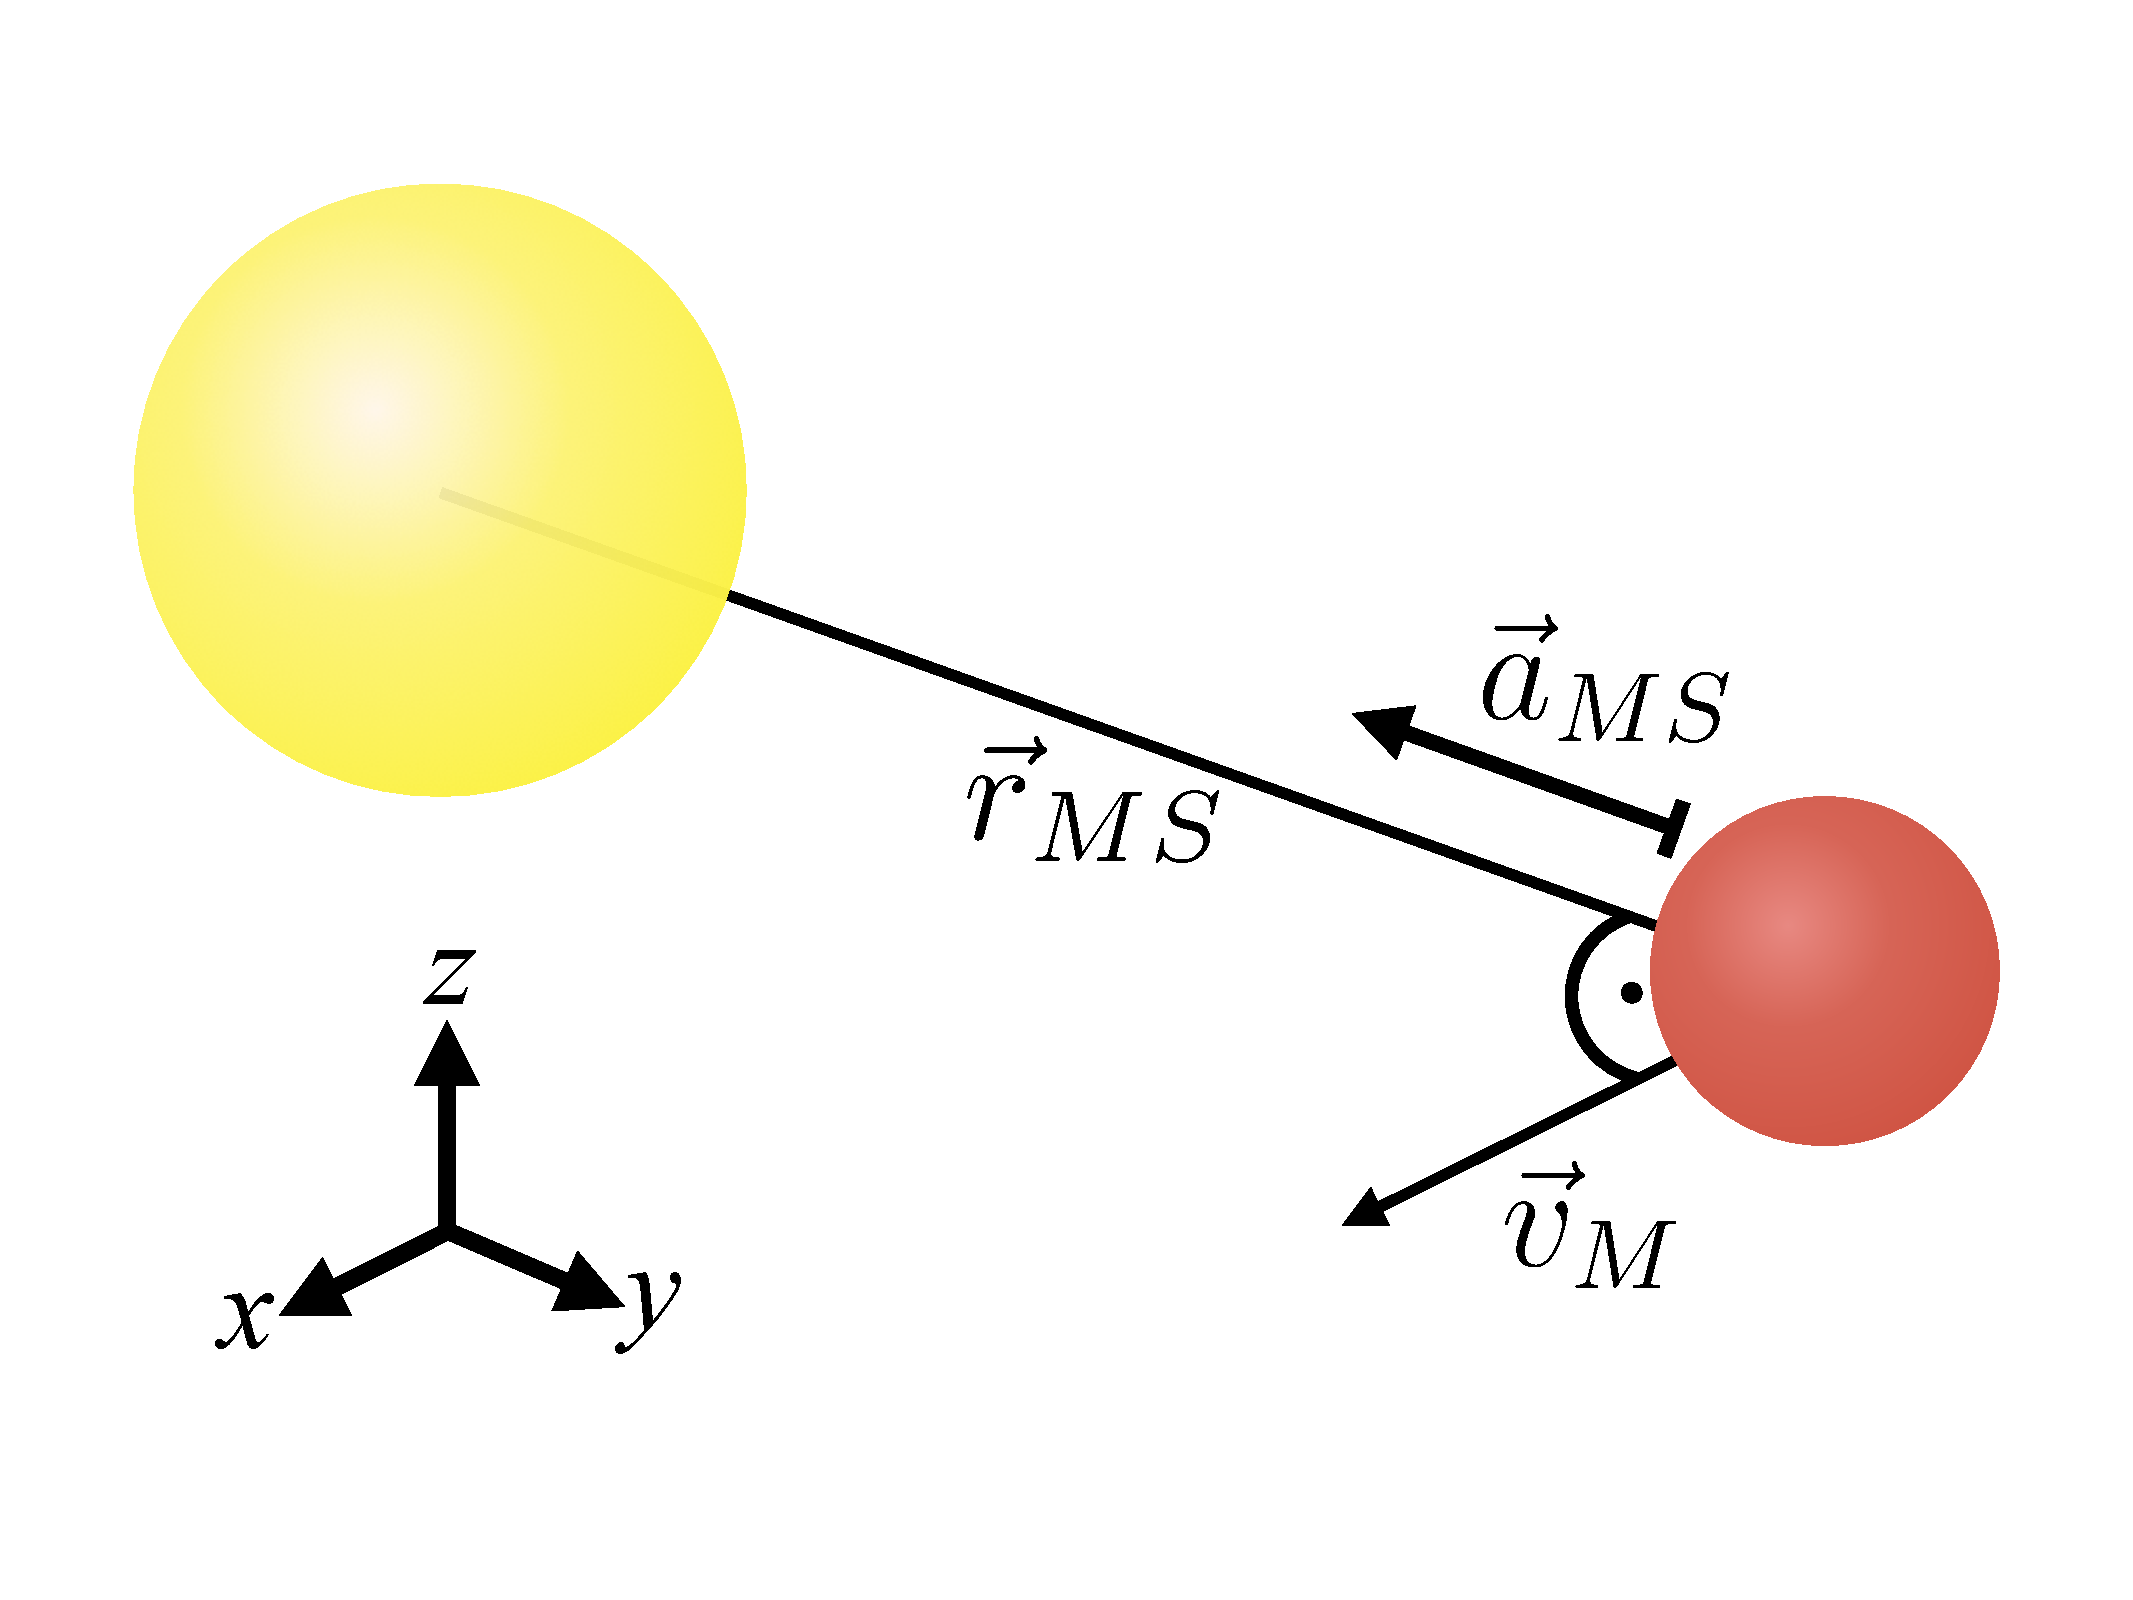
\includegraphics[width=.4\textwidth]{figs/sun_merc.pdf}
	\caption{\label{fig:sun_merc}Sun mercury system with relevant vectors.  Because the mercury is at its perihelion, its velocity is perpendicular to its direct connection vector with the sun.}
\end{figure}


In python, this reads
\begin{lstlisting}
	# Definition of parameters
	rM0 = 4.6    # in units of R0
	vM0 = 0.34   # in units of R0/T0
	aM  = 0.99   # in units of R0/T0**2
\end{lstlisting}
So far we only fixed the length of the vectors.
Next, we set up the initial directions, which will describe the motion in the two-dimensional plane.  We will build on the existing \python module \texttt{Vpython}, which provides  an implementation for treating vectors as well as their visualization.
The first object of interest is a \texttt{vector}, which takes three-dimensional coordinates as its input.  Because of our choice of initial conditions (we picked the initial vectors in the perihelion), the velocity of mercury is perpendicular to the vector which connects mercury and the sun (see figure \ref{fig:sun_merc}):
\begin{lstlisting}
	# Import the class vector from python
	from vpython import vector
	# Initialize distance and velocity vectors
	vec_rM0 = vector(0, rM0, 0)
	vec_vM0 = vector(vm0, 0, 0)
\end{lstlisting}
According to Eq.~(\ref{eq:newton}), the force which acts on mercury changes the velocity of mercury which eventually changes the position. However, we first need to fix the time step $\Delta t$ and use the estimate
of Eq.~(\ref{eq:check}) as a guidance {\bf Careful: Check units of dt}
\begin{lstlisting}
	# Definition of the time step
        dt = 2 * vm0 / aM / 100
\end{lstlisting}
Here the factor $1/100$ makes sure that $\Delta t$ is indeed
consistent with Eq.~(\ref{eq:check}).  {\bf We need to make sure that 'dt' is known
to the subroutines}
Now we are in the position to calculate
location and velocity of the planet at $t_0+\Delta t$ using the following comands
\begin{lstlisting}
	# Compute the strength of the acceleration
	aMS = aM * ( 1 + alpha * rS / vec_rM_old.mag  ) / vec_rM_old.mag**2
	# Multiply by the direction
	vec_aMS = - aMS * ( vec_rM_old / vec_rM_old.mag )
	# Update velocity vector
	vec_vM_new = vec_vM_old + vec_aMS * dt
	# Update position vector
	vec_rM_new = vec_rM_old + vec_vM_new * dt
\end{lstlisting}
Note the beauty of working with the predefined \texttt{vector} class: the basic vector operations are already implemented.  The difference and sum of two vectors, or the scalar vector multiplication return vectors themselves.  Also the magnitude of a vector -- \texttt{vector.mag} -- is a property of the vector and can be easily extracted.

It is handy to use \texttt{Python}s \texttt{function}s to embed repeating structures ("DRY" -- Don't Repeat Yourself)
\begin{lstlisting}
	# Define the function
	def evolve_mercury(vec_rM_old, vec_vM_old, alpha):
		<...Code...>
		return vec_rM_new, vec_vM_new
	
	# Call the function
	vec_rM_new, vec_vM_new = do_time_step(vec_rM_old, vec_vM_old)
\end{lstlisting}
Because of \python{$\!'$}s syntax, it is necessary that the body of the function is indented relative to the definition statement {\bf I do not understand this sentence}.

Finally, we can express the evolution by a \texttt{while}-loop
\begin{lstlisting}
	t = 0
	alpha=0
	# Execute the loop as long as t < T
	while t < T:
		vec_rM, vec_vM = evolve_mercury(vec_rM, vec_vM, alpha)
		t = t + dt
\end{lstlisting}
where for the start we set the parameter $\alpha$ to zero in order first study the properties of the pure 
$1/r^2$ force.
Note the required indent of the loop structure similar to the indent of a function.
In each iteration of the \texttt{while}-loop, the previous distance and velocity are used to compute the new values -- which directly overwrite the previous values and thus enter the next iteration.  The total runtime \texttt{T} is the amount of "virtual" days the simulations should run.
To describe at least one full orbit, $T$ needs to be larger than $T>..$.

{\bf Here we need to write something about visualizing the trajectories and how to run the code }

\section{Tests of stability}

\section{Tasks}


Ideas for questions:
\begin{itemize}
	\item Mass and motion of sun
	\item Estimate \texttt{dt} and also \texttt{T} in order to cover roughly two "mercury years".
	\item What does happen when you change those units?
	\item Compare values to the values in \cite{}.  Where does the difference come from?
	\item Start with $\alpha=0$. What do you observe?
\end{itemize}


\section{Dimensional analysis}

Dimensional analysis is not only a tool that allows one to cross check if the results of some simulation is
of the right order of magnitude, it is also very helpful to identify unusual dynamics in some system.
Especially the latter aspect should become clear from the discussion in this section.

The idea of dimensional analysis is that in a system that can be controlled by expanding the relevant quantities
(like the force) in some small parameter(s), the coefficients in the expansion should turn out to be of order unity (that
means anything between about 0.1 and 10 is fine - but 0.01 or 100 is irritating) --- parameters in line with this
are called 'natural'. Applied to the problem at hand
given by Eq.~(\ref{eq:newton}) this statement implies that from naturalness one would expect that 
the parameter $\alpha$ is of order 1 when one uses
for $r$ the average distance Mercury-sun, namely $\bar r=6\times 10^7$ km.
Form this one estimates for the expected angular shift per orbit
\begin{equation}
\delta \phi \simeq 2\pi\left(\frac{r_S}{\bar r}\right) = (\pi \times 10^{-7}) \ \mbox{rad} = (2\times 10^{-5})^o = (7\times 10^{-2}) ^{''} \ ,
\end{equation}
which leads to a shift of  about $30^{''}$ in 100 earth years to be compared to the empirical value of $43^{''}$.
 Thus indeed the
amount of perihelion motion of Mercury is in line with expectations, $if$ --- and this is an important 'if' ---
the Newtonian dynamics is simply the leading term of some more general underlying theory. In particular,
no new scales enter in the correction terms.

Thanks to Einstein we indeed know that the conclusion formulated above is correct ---- the more general underlying
theory is General Relativity and indeed Einstein was able to quantitatively explain the perihelion motion of Mercury
from his equations. 
On the other hand had we found a dramatic deviation of $\alpha$ from unity one would have concluded that 
there is probably some other dynamics going on that drives this difference.

Indeed, we now several of those hierarchy problems in modern physics: e.g. the so called QCD $\theta$ term,
expected to be of natural size, is at present known to be at most $10^{-10}$. This smallness, called the
strong CP problem, is so irritating that physicists like S. Weinberg even proposed that there must exist an
additional particle, the axion, whose interactions are in charge of pushing $\theta$ even to zero and there
are now intense searches for this axion going on various labs.

\section{Discussion of Starting Values}

\textit{I am not quite sure what to add here to Christopher's discussion.}\\

If the starting values are chosen as advised in the previous section, then the students should end up with a trajectory as depicted in figure \ref{fig:MercuryOrbit}. To get the perihelion motion, the term from equation \ref{eq:newton_art} has to be be added. This is a good opportunity to let the students play with the size of $\alpha$ and get a feeling for the impact on the trajectories. However it might be advisable to not start out with the correct mercury values but e.g. a slightly higher initial distance between mercury and sun, since the perihelion motion is better visible then. This is illustrated in figure \ref{fig:MercuryOrbit}, where we used a value of $\alpha=10^5$ and $dt=0.1T_0$.

\begin{figure}[htb]
	\centering
	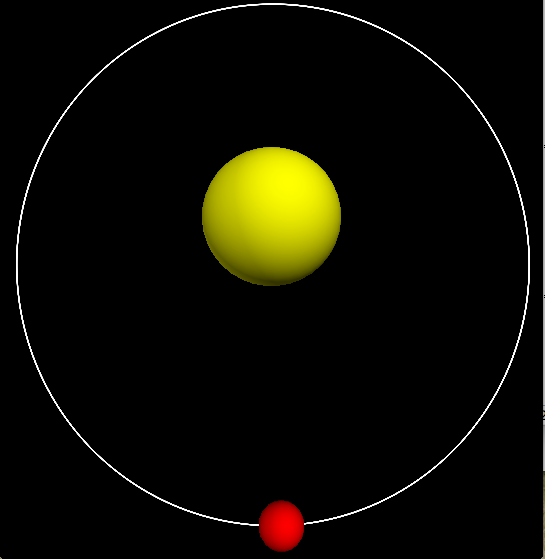
\includegraphics[width=.25\textwidth]{figs/MercuryOrbit.png} \quad
	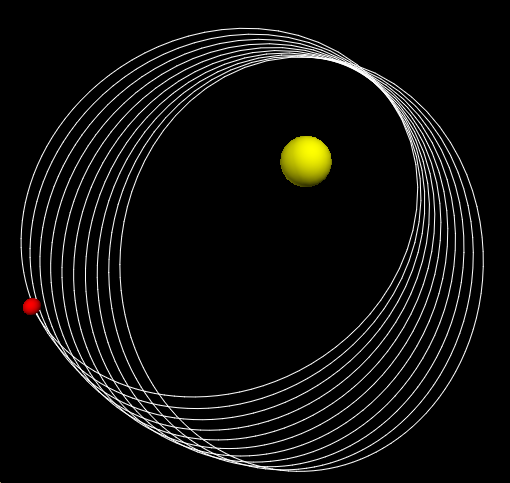
\includegraphics[width=.273\textwidth]{figs/PerihelionMotionLargeV.png} \quad
	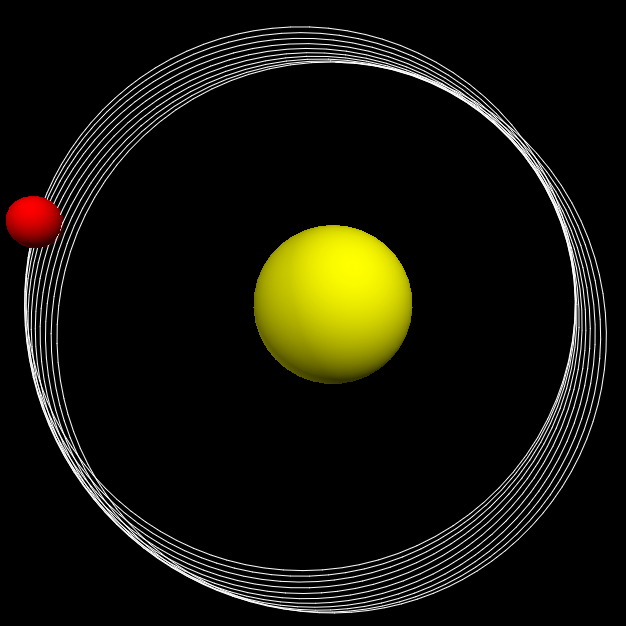
\includegraphics[width=.26\textwidth]{figs/PerihelionMotion.png}
	\caption{\label{fig:MercuryOrbit} Output for $\alpha=0$ (left), $\alpha=10^5$ and bigger starting distance $r_{MS}(0)=6R_0$ (middle) and $\alpha=10^5$ with original starting values.}
\end{figure}

\section{Extracting the Perihelion Motion}

\textit{What exactly do we want the students / advise the teachers to do? I think a nice approach would be to let the students implement the code to extract the perihelion motion and make a list of some values of alpha and the corresponding angles. Then discuss, that $\alpha=1$ is the natural size for $\alpha$ and that to extract the value of angle they need to exploit the linear dependence. Finally they can think on whether the value they get is reasonable and the teacher can explain the rest of section? What do you think?}\\

To calculate the expected size of the perihelion motion for a modified gravitational force, the students need to be abel to extract the angle. There are several ways to do this, but the easiest is to extract the point where the distance to the sun gets maximal, the aphelion, after $n$ turns and compare it to the original one. This can be done by using an $if$-statement in the $while$-loop.

Suppose we want to save the number of turns in the variable $counter$, the maximal number of turns in $maxcounter$ (here e.g. 10), the initial aphelion in the vector $a0$ and the final aphelion in the vector $a$. In addition to find out when the aphelion is reached, the last two positions $rlast$ and $rbeforelast$ have to be known. To set this up, before the while loop the following code needs to be included
\begin{lstlisting}
	r=r0
	rlast=r0
	counter=-1
	maxcounter=10
\end{lstlisting}
Then the following code needs to be included in the $while$-loop
\begin{lstlisting}
    rbeforelast=rlast
    rlast=r
    r=r+v*dt
    if (counter==-1): a0=rlast
    if (rbeforelast.mag<rlast.mag and rlast.mag>r.mag): counter=counter+1
    if counter==maxcounter:
    	a=rlast
    	break
\end{lstlisting}
and the condition for the $while$-loop should be set to $True$.
The angle between two vectors is given by the formula
 \begin{equation}
 	\sphericalangle(\vec{a}_0,\vec{a}) = \cos^{-1} \left( \frac{\vec{a}_0 \cdot \vec{a}}{|\vec{a}_0|\:|\vec{a}|} \right)
 \end{equation}
This is readily implemented in Vpython via
\begin{lstlisting}
	angle=acos(dot(a0,a)/(a0.mag*a.mag))/maxcounter*180/pi
	print("angle: ", (angle))
\end{lstlisting}

\begin{figure}[htb]
	\centering
	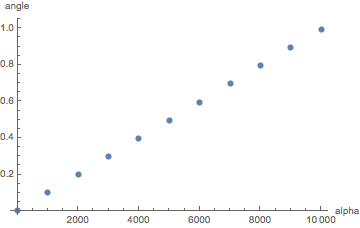
\includegraphics[width=.5\textwidth]{figs/AlphaAngle.png}
	\caption{\label{fig:AlphaAngle} Linear relation between $\alpha$ and the perihelion motion.}
\end{figure}

As explained above the natural value for $\alpha$ would be $1$. However if the student try out this value, they will find, that there is no visual change in the trajectories and the distance between the first an the last aphelion is of the order of magnitude of one step in the calculation $v_{aphelion}\cdot dt$. Therefore to estimate the size of the perihelion motion it is more advisable to use the fact, that there is an approximately linear dependence between $\alpha$ and the perihelion motion, if the angle is not to large. The students can convince themselves of this fact, by plotting some angles over $\alpha$. This can be done either by hand or using another program like e.g. Excel. One such plot can be found in figure \ref{fig:AlphaAngle}. Then to get to the angle at $\alpha=1$ one would ideally employ a line of best fit, but to get the order of magnitude right it is enough to consider only two points. Choosing $\alpha_1=1000$ and $\alpha_2=2000$ here, this would yield
\begin{equation}
	\Theta(\alpha=1) \approx \frac{0.201-0.100}{2000-1000} = 0.0001 = 0.36''
\end{equation}
so $3.63''\cdot 415\approx 150''$ per 100 earth years.
To find out, whether this is a reasonable result, the students could first follow the dimensional analysis and then compare to the actual value for the mercury  as outlined above.

\section{Possible extensions}

\begin{itemize}

\item \textbf{Explore Problem autonomously}

In chapter \ref{sec:Numerical Implementation} we suggested a certain way to present the material. By using a template as well as a step by step instruction, the students are guided rather strictly through the problem solution. We presented this approach with young students and limited time in mind. However if the students are more experienced and enough time is available, it is certainly advisable to give the students space for exploring the problem independently. This could be achieved by the following changes or additions to the concept presented in chapter \ref{sec:Numerical Implementation}

\begin{itemize}
\item \textbf{Build code from scratch}

Instead of providing the template to the students, they could build the program from scratch. Of course, this requires some basic knowledge in VPython, as they could acquire for example by working through a ball in the box example or the like. They could even look up the needed parameters on their own.
\item \textbf{Why can we work in one plane?}

In the code the third coordinate is never used. On the first glance, this could seem like a simplification. Let the students work out on their own, why this does not imply any loss of generality.
\item \textbf{What is the impact of the different parameters?}

Especially if the needed parameters are not specified beforehand, the students might have to experiment a bit, before getting the correct trajectories. But even if they are given, it might be beneficial to encourage the students to play with a few parameters, like mass or starting velocity, and track their impact on the trajectories. This way the students get a much better feeling for the physics involved.
\end{itemize}

\item \textbf{Optimizing performance}

Simulations always involve a balance between the time needed for the calculations and the accuracy of the results achieved. Even though this is a rather simple example, it contains some opportunities to make this concept accessible to the students.

\begin{itemize}
\item \textbf{Consider error due to finite time steps}

To make the students realise, that the finite time steps lead to inaccuracies in the trajectories encourage them to increase the time steps. This is best done in a program with unmodified gravitational force, as in this case the trajectories are closed ellipses and a deviation is most prominent. If the students choose the time steps big enough, they should witness big deviations. This exercise stresses the point, that by choosing increasingly smaller time steps, deviations from the physical trajectories can be reduced.
\item \textbf{Measure calculation time}

However in practice there is a limit to decreasing the time steps, because the time needed for the calculation grows simultaneously. By including
import time
\begin{lstlisting}
	start_time = time.time()
	main()
	print("--- %s seconds ---" % (time.time() - start_time))
\end{lstlisting}
the students can measure the time needed by their program. By varying dt they can validate, that there is indeed approximately an anti-proportional dependence. (Note: This only works if the time in the loop is increased by dt, so t=t+dt.)
\item \textbf{Verlet integration}

Of course by optimising the code, an improvement in accuracy can be achieved without increasing the calculation time. The simplest way to demonstrate this might be implementing Verlet integration instead of using the simple Euler method.
\end{itemize}

\item \textbf{Extended Problems}

\begin{itemize}
\item \textbf{Non-stationary sun}

It might be interesting to abandon the simplification of a stationary sun, as it nicely illustrates Newton's third law. Here it might also be advisable to reduce the mass of the sun to have a visible result.

\item \textbf{Three-body problem}

Ambitious students could even include another planet and see how the two planets interact. This is especially interesting, when discussing the perihelion motion of mercury, as it is mainly due to the influence of the other planets. Only a smaller part is due to general relativity.

\end{itemize}

\end{itemize}

%\begin{table}
%\caption{\label{jlab1}Journals to which this document applies, and macros for the abbreviated journal names in {\tt iopart.cls}. Macros for other journal titles are listed in appendix\,A.}
%\footnotesize
%\begin{tabular}{@{}llll}
%\br
%Short form of journal title&Macro name&Short form of journal title&Macro name\\
%\mr
%2D Mater.&\verb"\TDM"&Mater. Res. Express&\verb"\MRE"\\
%\br
%\end{tabular}\\
%$^{a}$UK spelling is required; $^{b}$MSC classification may be used as well as PACS; $^{c}$titles of articles are required in journal references; $^{d}$Harvard-style references must be used (see section \ref{except}); $^{e}$final page numbers of articles are required in journal references.
%
%\end{table}
%\normalsize

\subsection{Acknowledgments}
Here they come

\appendix
\section{Instructions to install V-phython}
\label{appendix:python}

\section{The code}
Here we should put the code
 

\bibliographystyle{alpha din}
\bibliography{MercuryNumerical}

\end{document}

